\pdfbookmark[0]{Forside}{label:forside}%
\begin{titlepage}
  \addtolength{\hoffset}{0.5\evensidemargin-0.5\oddsidemargin} %set equal margins on the frontpage - remove this line if you want default margins
  \noindent%
  \centering
  \begin{tabular}{@{}p{0.8\textwidth}@{}}
    \toprule[2pt]
    \midrule
    \vspace{0.2cm}
    \begin{center}
    \fontsize{32}{10}\selectfont{\textbf{
      Practical investigation of Rayleigh fading model in URC conditions  % insert your title here
    }}
    \end{center}
%    \begin{center}
%      \LARGE{
%      
%      }
%    \end{center}
    \vspace{0.2cm}\\
    \midrule
    \toprule[2pt]
  \end{tabular}  
  
  \centering

   %\vspace{0.55 cm}
\begin{figure}[H]
\centering
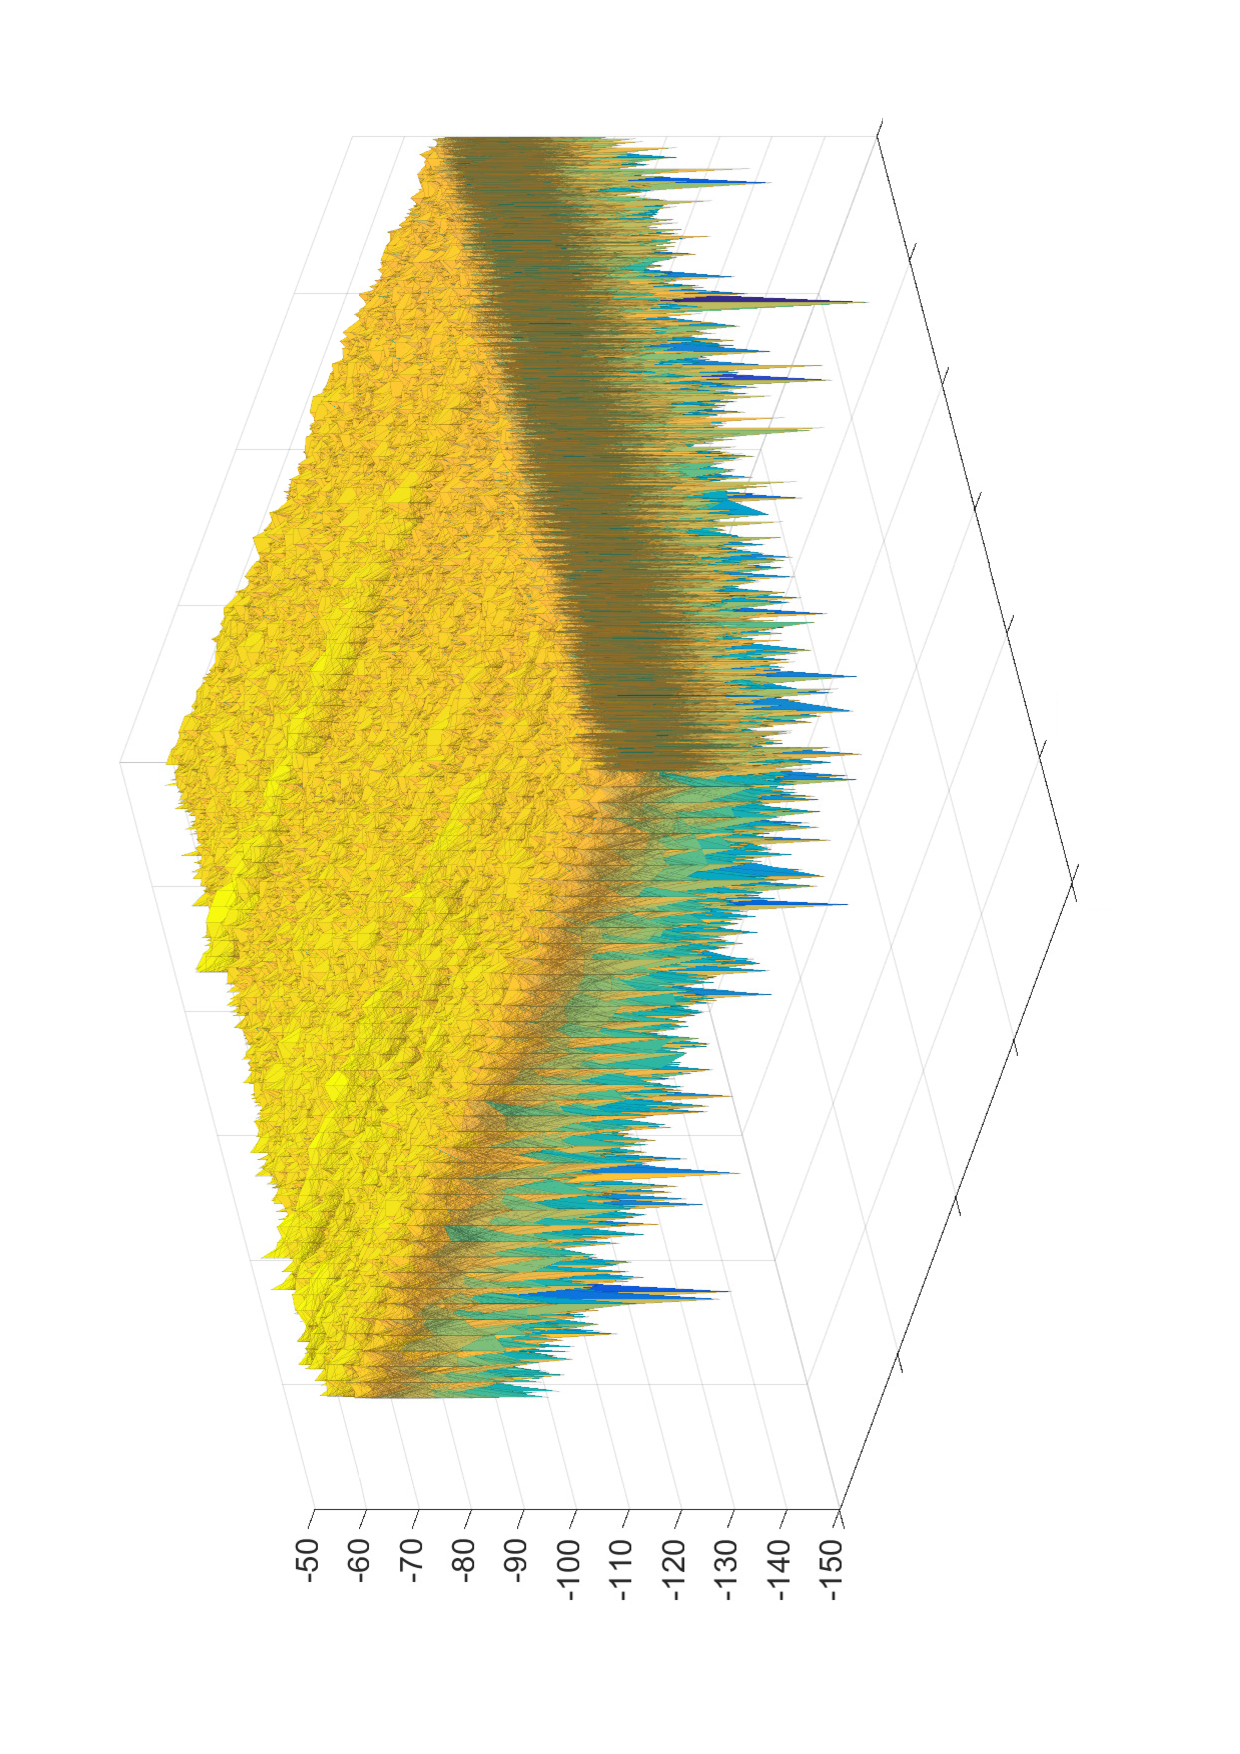
\includegraphics[height = 0.95\textwidth, angle = -90]{figures/Frontpage1.pdf}
%\label{fig:rawFadingMeas}
\end{figure}
\vfill
  \begin{center}
    {\large
      WCS8 project report %Insert document type (e.g., Project Report)
    }\\
    \vspace{0.2cm}
    {\Large
      Group 850%Insert your group name or real names here
    }
  \end{center}
  \vspace{1 cm}
%  \begin{center}
%  Aalborg University\\
%  Electronic Engineering \& IT\\
%  Frederiks Bajersvej 7\\
%  DK-9220 Aalborg
%  \end{center}
\end{titlepage}

\clearpage